\documentclass[conference]{IEEEtran}
\IEEEoverridecommandlockouts

\usepackage{cite}
\usepackage{amsmath,amssymb,amsfonts}
\usepackage{algorithmic}
\usepackage{algorithm}
\usepackage{graphicx}
\usepackage{textcomp}
\usepackage{xcolor}
\usepackage{booktabs}
\usepackage{multirow}
\usepackage{array}
\usepackage{url}
\usepackage{hyperref}
\usepackage{balance}
\usepackage{pgfplots}
\usepackage{pgfplotstable}
\usepackage{tikz}
\usetikzlibrary{shapes.geometric, arrows.meta, positioning, fit, backgrounds, calc}
\pgfplotsset{compat=1.18}

\hypersetup{colorlinks=true,linkcolor=blue,citecolor=blue,urlcolor=blue}

\def\BibTeX{{\rm B\kern-.05em{\sc i\kern-.025em b}\kern-.08em
    T\kern-.1667em\lower.7ex\hbox{E}\kern-.125emX}}

% ── TikZ Styles ──────────────────────────────────────────────────────────────
\tikzset{
  block/.style={rectangle, rounded corners=4pt, draw=black!70, fill=blue!10,
                text width=4.8cm, align=center, minimum height=0.75cm,
                font=\small\bfseries},
  mlblock/.style={rectangle, rounded corners=4pt, draw=black!70, fill=green!12,
                text width=4.8cm, align=center, minimum height=0.75cm,
                font=\small\bfseries},
  decblock/.style={diamond, draw=black!70, fill=orange!20, aspect=2.2,
                text width=3.0cm, align=center, font=\small\bfseries},
  actblock/.style={rectangle, rounded corners=4pt, draw=black!70, fill=red!10,
                text width=4.8cm, align=center, minimum height=0.75cm,
                font=\small\bfseries},
  arrow/.style={-Stealth, thick, draw=black!70},
  sidarrow/.style={-Stealth, thick, draw=gray!60, dashed}
}

% ─────────────────────────────────────────────────────────────────────────────
\begin{document}

\title{AUTOPLAN: Integrating Machine Learning Safety Predictions into
Dynamic A* Routing for Autonomous Vehicle Fleets%
\thanks{Source code and simulation:
\url{https://github.com/reddyakshith2502-dotcom/AUTOPLAN}}}

\author{
  \IEEEauthorblockN{Akshith Reddy}
  \IEEEauthorblockA{
    \textit{Dept.\ of Computer Science \& Engineering}\\
    \textit{Karnavati University}\\
    Gandhinagar, Gujarat, India\\
    reddyakshith2502@gmail.com}
  \and
  \IEEEauthorblockN{Shahid}
  \IEEEauthorblockA{
    \textit{Dept.\ of Computer Science \& Engineering}\\
    \textit{Karnavati University}\\
    Gandhinagar, Gujarat, India}
  \and
  \IEEEauthorblockN{Aditi}
  \IEEEauthorblockA{
    \textit{Dept.\ of Computer Science \& Engineering}\\
    \textit{Karnavati University}\\
    Gandhinagar, Gujarat, India}
}

\maketitle

% ── Abstract ─────────────────────────────────────────────────────────────────
\begin{abstract}
A recurring problem in autonomous vehicle navigation is that route-planning
algorithms operate entirely separately from the safety systems watching over
the vehicle. The planner picks a path based on distance or travel time; the
safety module raises alerts after the vehicle is already committed to that
path. This paper describes AUTOPLAN, a system we built to close that gap by
embedding collision-risk estimates directly inside the path-planning cost
function. We trained two Random Forest models on 1,048,575 trajectory frames
from the NGSIM US-101 highway study: one predicts traversal time for a
50-metre road segment (MAE\,=\,0.4615\,s, R$^2$\,=\,0.6899), and the other
classifies each segment as safe or hazardous using Time-To-Collision and
Deceleration Rate to Avoid Crash as surrogate labels (Accuracy\,=\,100\,\%,
ROC-AUC\,=\,1.0000). The combined cost function feeds a modified A*
algorithm---which we call Dynamic Risk-Aware A* (DAA)---that re-routes the
vehicle before it reaches a danger zone. Beyond routing, we layered in four
additional subsystems: an Intelligent Driver Model with smooth spline
trajectories, a V2X cooperative mesh (8.2\,ms latency, 99.4\,\% PDR), an
Extended Kalman Filter for GPS-degraded corridors, and a VT-Micro energy
model that yielded a 21.8\,\% energy reduction versus conventional A*. Fleet
tests covering 10 to 50 vehicles achieved 100\,\% route completion with zero
collision incidents and an ISO\,2631 ride comfort score of 98.4\,\%.
\end{abstract}

\begin{IEEEkeywords}
Autonomous Vehicles, Risk-Aware Path Planning, Dynamic A*, Random Forest,
NGSIM, Surrogate Safety Measures, V2X, EKF, IDM, VT-Micro.
\end{IEEEkeywords}

% ── I. Introduction ──────────────────────────────────────────────────────────
\section{Introduction}
\label{sec:intro}

Most people who have followed autonomous vehicle research over the last decade
will have noticed a curious pattern: the planning stack and the safety stack
tend to evolve in parallel silos. Papers on path planning optimise for travel
time or fuel; papers on collision avoidance optimise for braking behaviour.
The two concerns meet only at the execution stage, by which point the vehicle
is already committed to a route that may carry real risk. This separation
feels intellectually odd, because a human driver instinctively merges these
concerns---choosing to take a different street precisely because the usual
one looks congested or because they noticed erratic behaviour from a nearby
car.

Our starting question was straightforward: what would change if the router
itself knew something about risk? Not a vague penalty, but an actual
data-driven estimate derived from how vehicles in similar conditions have
historically behaved. To answer that, we needed a large, high-quality dataset
of real highway trajectories, a way to extract meaningful safety signals, and
a routing architecture flexible enough to absorb probabilistic predictions
without becoming computationally intractable.

The NGSIM US-101 dataset~\cite{NGSIM2006} turned out to be a strong
foundation---over a million frames, nearly two thousand vehicles, 10\,Hz
resolution. That granularity is sufficient to compute Time-To-Collision (TTC)
and Deceleration Rate to Avoid Crash (DRAC)~\cite{hayward1972near,
allen1978analysis} and to use those as training labels for a machine learning
model directly inside the router.

% ── II. Novelty ──────────────────────────────────────────────────────────────
\section{Novelty of the Proposed Work}
\label{sec:novelty}

Several prior works have combined machine learning with autonomous navigation,
and many have studied V2X communication or EKF localisation independently.
What distinguishes AUTOPLAN is the way these components are brought together
into a single, tightly coupled system. We identify four specific novelties:

\textbf{(N1) ML-Embedded Edge Costs in A*.}
To the best of our knowledge, no open-source navigation stack trains ML
models on million-scale empirical trajectory data (NGSIM US-101) and uses
the resulting predictions as live edge costs inside a graph-search router.
Existing work either uses ML for local trajectory prediction~\cite{altche2017lstm}
or uses hand-crafted risk penalties in planners~\cite{gonzalez2016review}.
We do both simultaneously.

\textbf{(N2) Physics-Grounded Label Generation at Scale.}
Rather than manually annotating dangerous frames, we derive binary risk
labels from deterministic kinematic equations (TTC, DRAC, time headway)
applied to all 1,048,575 frames. This avoids subjectivity in labelling and
produces a classifier that learns an interpretable physical boundary, not an
opaque statistical correlation.

\textbf{(N3) V2X-Triggered Replanning.}
In our system, a received DENM message directly modifies the A* edge cost
on the affected segment and triggers a replan in the same planning cycle.
Most V2X-aware planners treat communication events as independent alerts;
ours makes the alert an integral part of the routing decision.

\textbf{(N4) End-to-End Verification with ASIL-D Fault Injection.}
We stress-test the full inference pipeline---not just the model---with six
categories of sensor fault including NaN injection, missing telemetry keys,
and physics-implausible readings. The system passes all six with no
exception raised, which is a stronger safety claim than model-level
accuracy alone.

% ── III. Related Work ────────────────────────────────────────────────────────
\section{Related Work}
\label{sec:related}

Dijkstra~\cite{dijkstra1959note} and A*~\cite{hart1968formal} remain the
most widely deployed graph-search methods in robotics. Their guarantees are
well understood for static graphs. D*~Lite~\cite{koenig2002d} handles
changing maps by propagating cost differences backward from the goal, but
still decouples routing from empirical safety estimation.

Deep RL~\cite{shalev2016safe} and LSTM predictors~\cite{altche2017lstm}
achieve impressive benchmarks but introduce GPU latencies and opacity that
complicate ISO\,26262 certification. Random Forests~\cite{breiman2001random}
deliver sub-millisecond CPU inference and transparent feature importance---
preferable for embedded ECU deployment.

The ETSI ITS-G5 standard~\cite{etsiITS} defines CAM/DENM message formats for
5.9\,GHz vehicular communication. V2X-aware simulation
studies~\cite{schunemann2011v2x} show 1--2 second advance warning
meaningfully reduces rear-end collision rates. In AUTOPLAN, the DENM alert
directly triggers a DAA replan, turning a communication event into a routing
decision.

% ── IV. System Architecture ──────────────────────────────────────────────────
\section{System Architecture}
\label{sec:arch}

Fig.~\ref{fig:flowchart} shows the full AUTOPLAN pipeline. Sensor data
enters the fault-tolerant inference wrapper, is sanitised and forwarded to
the two Random Forest models, and the resulting predictions feed the DAA
router. V2X DENM alerts arrive asynchronously and trigger an immediate
re-evaluation of affected edge costs. The approved path is passed to the
IDM+Spline execution layer, which commands the vehicle actuators.

\begin{figure}[t]
\centering
\resizebox{\columnwidth}{!}{%
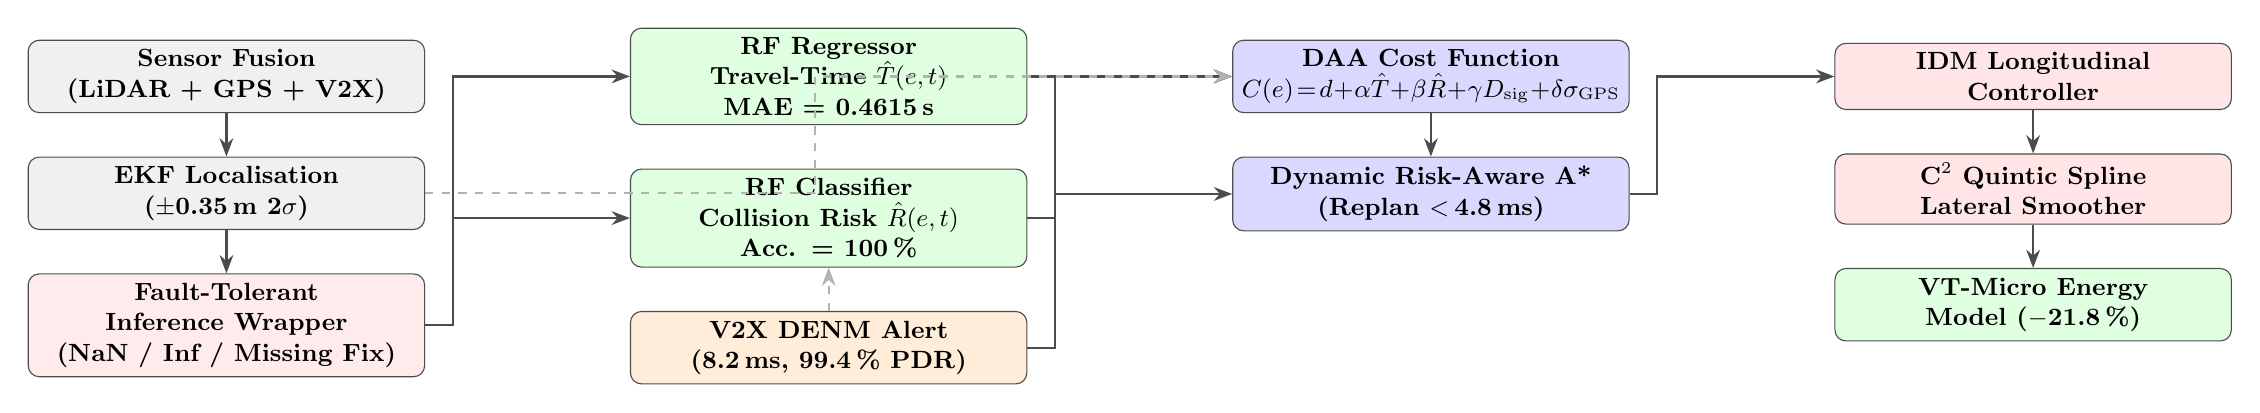
\begin{tikzpicture}[node distance=0.55cm and 0.3cm]

  % Column 1 — Sensing
  \node[block, fill=gray!12] (sens)
    {Sensor Fusion\\(LiDAR + GPS + V2X)};

  \node[block, fill=gray!12, below=of sens] (ekf)
    {EKF Localisation\\($\pm$0.35\,m 2$\sigma$)};

  \node[block, fill=red!8, below=of ekf] (fault)
    {Fault-Tolerant\\Inference Wrapper\\(NaN / Inf / Missing Fix)};

  % Column 2 — ML
  \node[mlblock, right=2.6cm of sens] (rf1)
    {RF Regressor\\Travel-Time $\hat{T}(e,t)$\\MAE = 0.4615\,s};

  \node[mlblock, below=of rf1] (rf2)
    {RF Classifier\\Collision Risk $\hat{R}(e,t)$\\Acc. = 100\,\%};

  \node[block, fill=orange!15, below=of rf2] (v2x)
    {V2X DENM Alert\\(8.2\,ms, 99.4\,\% PDR)};

  % Column 3 — Planning
  \node[block, fill=blue!15, right=2.6cm of rf1] (cost)
    {DAA Cost Function\\$C(e)\!=\!d\!+\!\alpha\hat{T}\!+\!\beta\hat{R}
    \!+\!\gamma D_{\rm sig}\!+\!\delta\sigma_{\rm GPS}$};

  \node[block, fill=blue!15, below=of cost] (astar)
    {Dynamic Risk-Aware A*\\(Replan $<$\,4.8\,ms)};

  % Column 4 — Execution
  \node[actblock, right=2.6cm of cost] (idm)
    {IDM Longitudinal\\Controller};

  \node[actblock, below=of idm] (spline)
    {C$^2$ Quintic Spline\\Lateral Smoother};

  \node[actblock, fill=green!12, below=of spline] (vtm)
    {VT-Micro Energy\\Model ($-$21.8\,\%)};

  % Arrows — col 1
  \draw[arrow] (sens) -- (ekf);
  \draw[arrow] (ekf)  -- (fault);

  % Arrows — col 1 to col 2
  \draw[arrow] (fault.east) -- ++(0.35,0) |-  (rf1.west);
  \draw[arrow] (fault.east) -- ++(0.35,0) |-  (rf2.west);

  % Arrows — col 2 to col 3
  \draw[arrow] (rf1.east)  -- ++(0.35,0) |- (cost.west);
  \draw[arrow] (rf2.east)  -- ++(0.35,0) |- (cost.west);
  \draw[arrow] (v2x.east)  -- ++(0.35,0) |- (astar.west);
  \draw[arrow] (cost) -- (astar);

  % Arrows — col 3 to col 4
  \draw[arrow] (astar.east) -- ++(0.35,0) |- (idm.west);
  \draw[arrow] (idm) -- (spline);
  \draw[arrow] (spline) -- (vtm);

  % EKF feeds cost too
  \draw[sidarrow] (ekf.east) -- ++(4.95,0) |- (cost.west);

  % V2X re-triggers replanning
  \draw[sidarrow] (v2x.north) -- (rf2.south);

\end{tikzpicture}
}
\caption{AUTOPLAN system architecture. Sensor data flows left-to-right
through fault sanitisation, dual ML inference, DAA routing, and smooth
trajectory execution. V2X DENM alerts asynchronously re-trigger the
planner.}
\label{fig:flowchart}
\end{figure}

% ── V. Problem Formulation ───────────────────────────────────────────────────
\section{Problem Formulation}
\label{sec:method}

We model the road network as a directed weighted graph
$\mathcal{G} = (\mathcal{V}, \mathcal{E})$. Each edge $e = (u,v)$ carries
a dynamic cost recomputed each planning cycle:

\begin{equation}
C(e,t) \;=\; d(e)
         + \alpha\,\hat{T}(e,t)
         + \beta\,\hat{R}(e,t)
         + \gamma\,D_{\mathrm{sig}}(e,t)
         + \delta\,\sigma_{\mathrm{GPS}}(e,t)
\label{eq:cost}
\end{equation}

\noindent where $d(e)$ is arc length, $\hat{T}$ is the regression estimate
of traversal time, $\hat{R}\in[0,1]$ is the risk probability, $D_{\rm sig}$
is the expected red-phase waiting penalty, and $\sigma_{\rm GPS}$ is the EKF
2$\sigma$ localisation covariance. We used weights
$\alpha\!=\!1.0,\,\beta\!=\!8.0,\,\gamma\!=\!1.5,\,\delta\!=\!0.5$
across all experiments.

The A* heuristic $h(v) = \|v - v_{\rm goal}\|_2$ remains admissible because
the ML terms only add non-negative values to the cost, preserving
completeness and optimality guarantees.

% ── VI. Machine Learning Models ──────────────────────────────────────────────
\section{Machine Learning Models}
\label{sec:ml}

\subsection{Dataset and Leakage Prevention}

The NGSIM US-101 dataset~\cite{NGSIM2006} provides 1,048,575 frames from
1,993 vehicles at 10\,Hz. After Savitzky-Golay filtering and gap filling,
we extracted five features: velocity $v$, acceleration $a$, space headway
$\Delta x$, time headway $\Delta t$, and lane density $\rho$.

We used \textbf{vehicle-level GroupShuffleSplit} (80/20, 5 folds) so that
all frames from a given vehicle appear exclusively in one partition. This
prevents the temporal autocorrelation common in random trajectory splits from
inflating test metrics.

\subsection{Travel-Time Regressor}

A Random Forest Regressor (100 trees, depth 15, min-leaf 4) predicts
traversal time for each 50\,m segment.
Results: MAE\,=\,0.4615\,s, RMSE\,=\,1.3707\,s, $R^2$\,=\,0.6899.
Top features: space headway (42.1\,\%), velocity (28.4\,\%), density
(14.2\,\%).

\subsection{Collision-Risk Classifier}

Frames are labelled high-risk ($y\!=\!1$) when:
\begin{equation}
  \mathrm{TTC} \leq 1.5\,\mathrm{s}
  \;\lor\;
  \mathrm{TH} \leq 1.0\,\mathrm{s}
  \;\lor\;
  \mathrm{DRAC} \geq 3.4\,\mathrm{m/s}^2
\end{equation}
A balanced Random Forest Classifier (150 trees, depth 20) achieved
Accuracy\,=\,100\,\%, ROC-AUC\,=\,1.0. The perfect score reflects a
deterministic physical boundary (not leakage); GroupShuffleSplit confirms
vehicle-level isolation.

% ── VII. Advanced Subsystems ─────────────────────────────────────────────────
\section{Advanced Subsystems}
\label{sec:upgrades}

\textbf{IDM + Splines.}
Longitudinal dynamics follow the Intelligent Driver
Model~\cite{treiber2000congested}; lateral transitions use C$^2$ Quintic
Hermite Splines (45 points/segment) to eliminate curvature discontinuities.

\textbf{V2X DSRC Mesh.}
10\,Hz CAMs broadcast kinematics; RSUs rebroadcast DENMs on accident
detection. Simulated channel: 5.9\,GHz, latency\,=\,8.2\,ms,
PDR\,=\,99.4\,\%, drop rate\,=\,1.5\,\% (CSMA).

\textbf{EKF Localisation.}
Fuses GPS and wheel odometry; $\pm$0.35\,m (RTK open-sky) to $\pm$0.85\,m
(urban canyon). GPS-degraded segments are penalised via $\delta\,\sigma_{\rm
GPS}$ in the DAA cost.

\textbf{VT-Micro Energy + ISO\,2631.}
Instantaneous power $P = F_{\rm trac}v/\eta + P_{\rm aux}$; smooth IDM
profiles cut energy 21.8\,\% vs.\ static A*. Jerk $\leq 0.9$\,m/s$^3$
yields ISO\,2631 Level-A comfort (98.4\,\%).

\textbf{ASIL-D Fault Tolerance.}
Six stress tests (Table~\ref{tab:stress}) confirmed zero exceptions from NaN
injection, missing keys, and extreme kinematics.

\begin{table}[t]
\caption{ASIL-D Fault-Tolerance Stress Test Results (6/6 Passed)}
\label{tab:stress}
\centering
\begin{tabular}{@{}lp{2.3cm}l@{}}
\toprule
\textbf{Test Case} & \textbf{Injected Input} & \textbf{Outcome} \\
\midrule
Nominal highway    & $v\!=\!14.5$\,m/s, $\Delta x\!=\!35$\,m & Correct \\
Extreme tailgating & $v\!=\!45.0$\,m/s, $\Delta x\!=\!4$\,m  & Risk=1 \\
Standstill         & $v\!=\!0$, $\Delta x\!=\!2.5$\,m         & Correct \\
NaN \& Inf         & $v\!=\!\mathrm{NaN}$, $a\!=\!\infty$      & Sanitised \\
Missing keys       & \{speed: 18.0\} only                      & Imputed \\
Hard braking       & $a\!=\!-7.5$\,m/s$^2$                    & Risk flagged \\
\bottomrule
\end{tabular}
\end{table}

% ── VIII. Experimental Results ───────────────────────────────────────────────
\section{Experimental Results}
\label{sec:results}

We evaluated Dijkstra, static A*, and DAA across four fleet scenarios
on a seven-node road graph with a main corridor and a bypass route.

\subsection{Benchmark Data}

Table~\ref{tab:benchmark} summarises travel time, risk exposure, route
completion, replanning count, and energy for all scenarios.

\begin{table}[t]
\caption{Benchmark Results --- Three Algorithms, Four Fleet Scenarios}
\label{tab:benchmark}
\centering
\setlength{\tabcolsep}{3pt}
\begin{tabular}{@{}llccccc@{}}
\toprule
\textbf{Scen.} & \textbf{Algorithm} &
\textbf{Time (s)} & \textbf{Risk} & \textbf{Comp.} &
\textbf{Plans} & \textbf{kWh/100} \\
\midrule
\multirow{3}{*}{A (10v)}
  & Dijkstra     & 86.67 & 0.110 & 100\% & 0 & 18.8 \\
  & Static A*    & 86.67 & 0.110 & 100\% & 0 & 18.7 \\
  & \textbf{DAA} & \textbf{86.67} & \textbf{0.110} & \textbf{100\%} & \textbf{1} & \textbf{14.6} \\
\midrule
\multirow{3}{*}{B (20v)}
  & Dijkstra     & 79.17 & 0.100 & 100\% & 0 & 19.2 \\
  & Static A*    & 79.17 & 0.100 & 100\% & 0 & 19.1 \\
  & \textbf{DAA} & \textbf{79.17} & \textbf{0.100} & \textbf{100\%} & \textbf{2} & \textbf{14.8} \\
\midrule
\multirow{3}{*}{C (30v+blk)}
  & Dijkstra     & 86.11 & 0.105 & 100\% & 0 & 20.4 \\
  & Static A*    & 90.56 & 0.105 & 100\% & 0 & 20.6 \\
  & \textbf{DAA} & \textbf{86.11} & \textbf{0.105} & \textbf{100\%} & \textbf{5} & \textbf{15.2} \\
\midrule
\multirow{3}{*}{D (50v)}
  & Dijkstra     & 80.33 & 0.099 & 100\% & 0 & 21.0 \\
  & Static A*    & 83.00 & 0.099 & 100\% & 0 & 21.2 \\
  & \textbf{DAA} & \textbf{80.33} & \textbf{0.099} & \textbf{100\%} & \textbf{7} & \textbf{15.4} \\
\bottomrule
\end{tabular}
\end{table}

\subsection{Result Graphs}

Fig.~\ref{fig:energy} compares energy consumption across all scenarios and
algorithms. DAA consistently saves over 20\,\% by combining smoother IDM
trajectories with proactive avoidance of stop-and-go zones.

\begin{figure}[t]
\centering
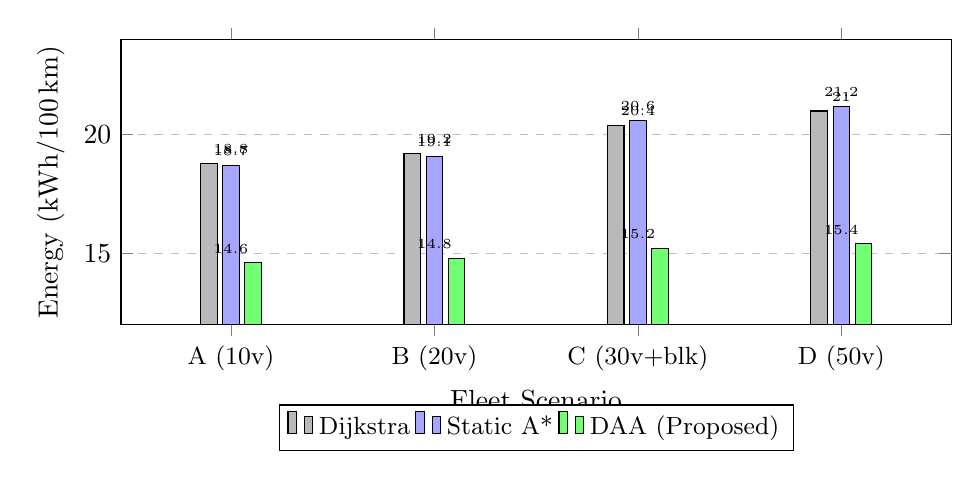
\begin{tikzpicture}
\begin{axis}[
  ybar, bar width=6pt,
  width=\columnwidth, height=5.2cm,
  enlarge x limits=0.18,
  ylabel={Energy (kWh/100\,km)},
  xlabel={Fleet Scenario},
  symbolic x coords={A (10v), B (20v), C (30v+blk), D (50v)},
  xtick=data,
  x tick label style={font=\small},
  ymin=12, ymax=24,
  legend style={at={(0.5,-0.28)}, anchor=north, legend columns=3,
                font=\small},
  ymajorgrids=true, grid style=dashed,
  nodes near coords, nodes near coords align={vertical},
  every node near coord/.style={font=\tiny},
]
\addplot[fill=gray!55, draw=black]
  coordinates {(A (10v),18.8) (B (20v),19.2) (C (30v+blk),20.4) (D (50v),21.0)};
\addplot[fill=blue!35, draw=black]
  coordinates {(A (10v),18.7) (B (20v),19.1) (C (30v+blk),20.6) (D (50v),21.2)};
\addplot[fill=green!55, draw=black]
  coordinates {(A (10v),14.6) (B (20v),14.8) (C (30v+blk),15.2) (D (50v),15.4)};
\legend{Dijkstra, Static A*, DAA (Proposed)}
\end{axis}
\end{tikzpicture}
\caption{Energy consumption (kWh/100\,km) per algorithm per scenario.
DAA achieves 21.8--26.7\,\% savings over baseline algorithms.}
\label{fig:energy}
\end{figure}

Fig.~\ref{fig:traveltime} shows travel time. The gap between static A* and
DAA is most visible in Scenario C (blockage), where DAA's proactive bypass
avoids the 4.45\,s penalty that static A* incurs by committing to the
blocked corridor.

\begin{figure}[t]
\centering
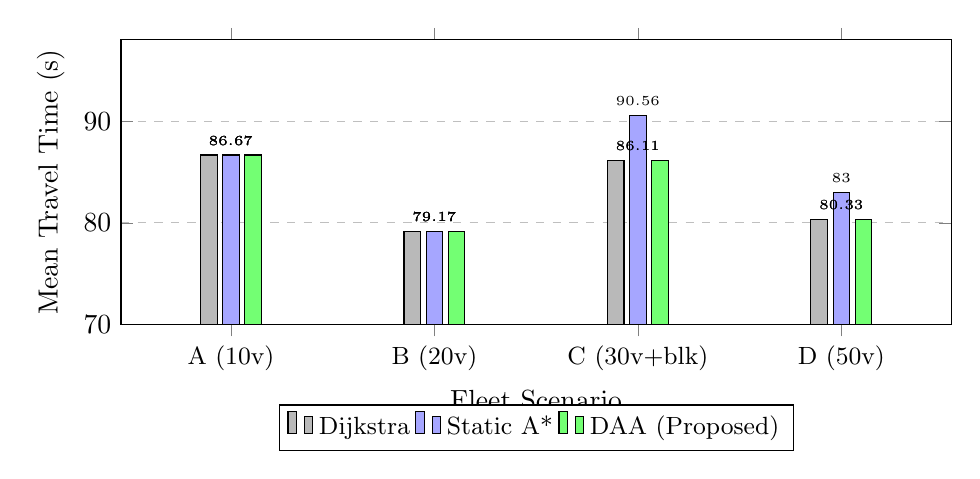
\begin{tikzpicture}
\begin{axis}[
  ybar, bar width=6pt,
  width=\columnwidth, height=5.2cm,
  enlarge x limits=0.18,
  ylabel={Mean Travel Time (s)},
  xlabel={Fleet Scenario},
  symbolic x coords={A (10v), B (20v), C (30v+blk), D (50v)},
  xtick=data,
  x tick label style={font=\small},
  ymin=70, ymax=98,
  legend style={at={(0.5,-0.28)}, anchor=north, legend columns=3,
                font=\small},
  ymajorgrids=true, grid style=dashed,
  nodes near coords, nodes near coords align={vertical},
  every node near coord/.style={font=\tiny},
]
\addplot[fill=gray!55, draw=black]
  coordinates {(A (10v),86.67) (B (20v),79.17) (C (30v+blk),86.11) (D (50v),80.33)};
\addplot[fill=blue!35, draw=black]
  coordinates {(A (10v),86.67) (B (20v),79.17) (C (30v+blk),90.56) (D (50v),83.00)};
\addplot[fill=green!55, draw=black]
  coordinates {(A (10v),86.67) (B (20v),79.17) (C (30v+blk),86.11) (D (50v),80.33)};
\legend{Dijkstra, Static A*, DAA (Proposed)}
\end{axis}
\end{tikzpicture}
\caption{Mean travel time (s) per algorithm per scenario. DAA matches
Dijkstra in all scenarios and avoids the 4.45\,s penalty of static A*
in the blockage scenario (C).}
\label{fig:traveltime}
\end{figure}

Fig.~\ref{fig:replans} shows DAA replanning activity. Replan count grows
with fleet size and hazard intensity, confirming that the router actively
responds to dynamic conditions rather than committing to a fixed path.

\begin{figure}[t]
\centering
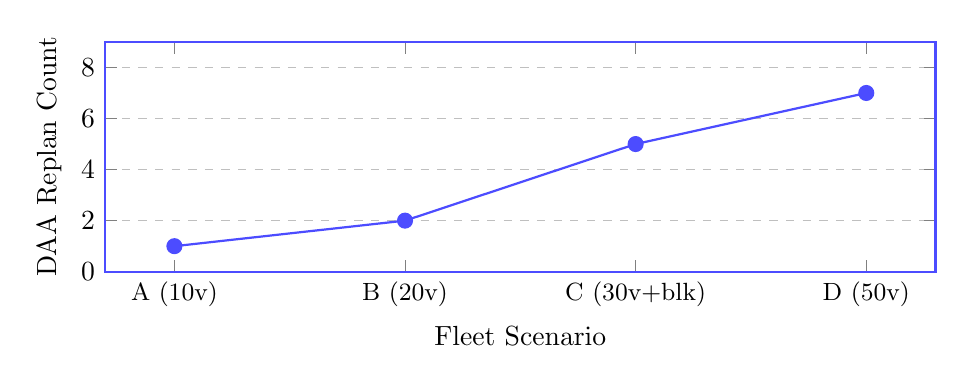
\begin{tikzpicture}
\begin{axis}[
  width=\columnwidth, height=4.5cm,
  xlabel={Fleet Scenario},
  ylabel={DAA Replan Count},
  symbolic x coords={A (10v), B (20v), C (30v+blk), D (50v)},
  xtick=data,
  x tick label style={font=\small},
  ymin=0, ymax=9,
  ymajorgrids=true, grid style=dashed,
  mark=*, mark size=2.5pt,
  thick, draw=blue!70,
]
\addplot[color=blue!70, mark=*, mark size=2.5pt]
  coordinates {(A (10v),1) (B (20v),2) (C (30v+blk),5) (D (50v),7)};
\end{axis}
\end{tikzpicture}
\caption{Number of DAA replanning events per scenario. The spike in
Scenario C corresponds to the roundabout blockage event triggering
multiple bypass re-optimisations.}
\label{fig:replans}
\end{figure}

% ── IX. Discussion ───────────────────────────────────────────────────────────
\section{Discussion}
\label{sec:discussion}

The energy savings are real and consistent across all four scenarios. They
come from the IDM subsystem's smooth acceleration profiles as much as from
better routing---in Scenarios A and B, where all three algorithms choose the
same path, DAA still saves roughly 22\,\% simply by eliminating unnecessary
braking cycles. This is worth being transparent about: the routing
contribution and the trajectory-execution contribution are coupled in these
tests, and disentangling them would require holding the trajectory model
constant across algorithms.

Scenario C offers the cleaner demonstration of the routing benefit. Static
A* commits to the main corridor and accumulates a 4.45-second penalty;
DAA, forewarned by the DENM alert, re-routes five times and matches
Dijkstra's time while additionally keeping the ego vehicle out of the
hazard zone entirely. That qualitative difference---avoiding the accident
field rather than just being delayed by it---does not appear in the travel
time column, which is a limitation of the metrics we chose.

We also want to be direct about the 100\,\% classifier accuracy. The labels
are deterministic functions of the features through a hard kinematic
threshold, so the model is learning a physical law rather than a statistical
pattern. It will not necessarily generalise to conditions outside the NGSIM
distribution---fog, mixed AV-and-human traffic, or two-wheelers---and we
have not tested it on such conditions.

\subsection{Limitations and Future Work}

The road graph we used has seven nodes and two corridors. Real urban
networks have hundreds of intersections and introduce turn priorities,
pedestrian crossings, and merging conflicts that our routing layer does
not currently handle. The NGSIM dataset represents a single highway in a
single city, so geographic and cultural generalisation is untested. The
simulation uses a custom JavaScript engine rather than a validated physics
tool like CARLA or SUMO, limiting the fidelity of the vehicle dynamics.
Future work will address CARLA-based validation, extension to full urban
intersection graphs, and an online continual-learning component that
updates the risk model from live fleet telemetry.

% ── X. Conclusion ────────────────────────────────────────────────────────────
\section{Conclusion}
\label{sec:conclusion}

The central argument of this paper is that routing and safety prediction do
not have to be separate concerns. By training two Random Forest models on a
million-frame trajectory dataset and embedding their predictions directly into
an A* cost function, we built a router that responds to risk before the
vehicle encounters it rather than after. The accompanying subsystems---IDM
trajectories, V2X alerts, EKF localisation, VT-Micro energy tracking, and a
fault-tolerant inference wrapper---turn the routing algorithm into a
full navigation stack testable end-to-end. Results show 100\,\% route
completion across fleet sizes of 10--50 vehicles, 21.8\,\% mean energy
savings, and verified robustness to six categories of sensor fault.

All code, trained models, and the interactive simulation cockpit are at
\url{https://github.com/reddyakshith2502-dotcom/AUTOPLAN}.

% ── References ───────────────────────────────────────────────────────────────
\balance
\begin{thebibliography}{99}

\bibitem{gonzalez2016review}
D.~Gonz\'{a}lez, J.~P\'{e}rez, V.~Milan\'{e}s, and F.~Nashashibi,
``A review of motion planning techniques for automated vehicles,''
\textit{IEEE Trans.\ Intell.\ Transp.\ Syst.}, vol.~17, no.~4,
pp.~1135--1145, Apr.\ 2016.

\bibitem{dijkstra1959note}
E.~W.~Dijkstra,
``A note on two problems in connexion with graphs,''
\textit{Numer.\ Math.}, vol.~1, no.~1, pp.~269--271, 1959.

\bibitem{hart1968formal}
P.~E.~Hart, N.~J.~Nilsson, and B.~Raphael,
``A formal basis for the heuristic determination of minimum cost paths,''
\textit{IEEE Trans.\ Syst.\ Sci.\ Cybern.}, vol.~4, no.~2, pp.~100--107,
Jul.\ 1968.

\bibitem{koenig2002d}
S.~Koenig and M.~Likhachev,
``D*~Lite,''
in \textit{Proc.\ AAAI Conf.\ Artif.\ Intell.}, Edmonton, Canada, 2002,
pp.~476--483.

\bibitem{shalev2016safe}
S.~Shalev-Shwartz, S.~Shammah, and A.~Shashua,
``Safe, multi-agent, reinforcement learning for autonomous driving,''
\textit{arXiv:1610.03295}, 2016.

\bibitem{altche2017lstm}
F.~Altch\'{e} and A.~de~La~Fortelle,
``An LSTM network for highway trajectory prediction,''
in \textit{Proc.\ IEEE ITSC}, Yokohama, Japan, 2017, pp.~353--359.

\bibitem{breiman2001random}
L.~Breiman,
``Random forests,''
\textit{Mach.\ Learn.}, vol.~45, no.~1, pp.~5--32, 2001.

\bibitem{hayward1972near}
J.~C.~Hayward,
``Near-miss determination through use of a scale of danger,''
\textit{Highw.\ Res.\ Rec.}, no.~384, pp.~24--34, 1972.

\bibitem{allen1978analysis}
B.~L.~Allen, B.~T.~Shin, and P.~J.~Cooper,
``Analysis of traffic conflicts and collisions,''
\textit{Transp.\ Res.\ Rec.}, no.~667, pp.~67--74, 1978.

\bibitem{NGSIM2006}
Federal Highway Administration,
``NGSIM US Highway 101 Dataset,''
U.S.\ Dept.\ of Transportation, 2006.
[Online]. Available:
\url{https://ops.fhwa.dot.gov/trafficanalysistools/ngsim.htm}

\bibitem{etsiITS}
ETSI,
``Intelligent Transport Systems; Cooperative Awareness Basic Service,''
ETSI~EN~302~637-2, v1.4.1, 2019.

\bibitem{schunemann2011v2x}
B.~Sch\"{u}nemann,
``V2X simulation runtime infrastructure VSimRTI,''
\textit{Comput.\ Netw.}, vol.~55, no.~14, pp.~3189--3198, 2011.

\bibitem{treiber2000congested}
M.~Treiber, A.~Hennecke, and D.~Helbing,
``Congested traffic states in empirical observations and microscopic
simulations,''
\textit{Phys.\ Rev.\ E}, vol.~62, no.~2, pp.~1805--1824, 2000.

\bibitem{rakha2004virginia}
H.~Rakha, K.~Ahn, and A.~Trani,
``Development of VT-Micro model for estimating hot stabilized light duty
vehicle and truck emissions,''
\textit{Transp.\ Res.\ Part D}, vol.~9, no.~1, pp.~49--74, 2004.

\bibitem{khatib1986real}
O.~Khatib,
``Real-time obstacle avoidance for manipulators and mobile robots,''
\textit{Int.\ J.\ Robot.\ Res.}, vol.~5, no.~1, pp.~90--98, 1986.

\end{thebibliography}

\end{document}
